%        File: DesignDocument.tex
%     Created: 一 3月 26 01:00 下午 2018 C
% Last Change: 一 3月 26 01:00 下午 2018 C
%
\documentclass[UTF8,noindent]{ctexart}
\usepackage[a4paper,left=2.0cm,right=2.0cm,top=2.0cm,bottom=2.0cm]{geometry}
\usepackage{hyperref}
\usepackage{url}
\usepackage{graphicx}
\usepackage{amsmath}
\usepackage{amssymb}
\usepackage{enumitem}
\usepackage{tikz}
\usepackage{float}
\usepackage{xeCJK}
\usepackage{listings}
\usepackage{xcolor}
\lstset{language = c,numbers=left, showstringspaces=false,keywordstyle= \color{ blue!70 },commentstyle=\color{red!50!green!50!blue!50}, frame=shadowbox, rulesepcolor= \color{ red!20!green!20!blue!20 } 
} 
\CTEXsetup[format={\Large\bfseries}]{section}
\usetikzlibrary{graphs}
%\newtheorem*{lemma}{Lemma}
\title{\CJKfamily{zhkai}计算机网络研讨课实验报告}
\author{{\CJKfamily{zhkai}冯吕}\ $2015K8009929049$}
\date{\today}
\begin{document}
\maketitle
\zihao{5}
\CJKfamily{zhsong}
%\begin{center}
%  \begin{tabular}{|p{15cm}|}
%    \hline
\section*{{\CJKfamily{zhhei}实验题目}}网络路由实验二
%\hline
\section*{{\CJKfamily{zhhei}实验内容}}
在本次实验中,需要基于上一次实验生成一致性链路数据库基础上,计算路由器表项。

计算路由器表项时,使用$Dijkstra$算法。
\section*{{\CJKfamily{zhhei}实验流程}}
在计算路由器表项时,分如下三步进行:
\begin{itemize}
  \item 将上一实验得到的一致状态链路数据库抽象成拓扑图;
	\item 利用生成的拓扑图通过$Dijkstra$算法计算最短路径;
	  \item 根据最短路径生成路由表项;
\end{itemize}
\subsection*{构建拓扑图}
构建网络拓扑图时,使用一个二维数组存储边,使用一个一维数组存储节点。

构建网络拓扑图的函数为:$caculate\_graph$
\begin{lstlisting}
static int caculate_graph(){
	int node_num =  0;
	int x, y;
	mospf_db_entry_t *db_pos, *db_q;
	init_Graph();
	Node[node_num++] = instance->router_id;
	if (list_empty(&mospf_db)){
		printf("Emmty Database.\n");
		return node_num;
	}
	list_for_each_entry_safe(db_pos, db_q, &mospf_db, list){
		Node[node_num++] = db_pos->rid;
	}
	list_for_each_entry_safe(db_pos, db_q, &mospf_db, list){
		for(int i = 0; i != db_pos->nadv; ++i){
			x = get_Node(db_pos->array[i].rid, node_num);
			y = get_Node(db_pos->rid, node_num);
			Graph[x][y] = Graph[y][x] = 1;
		}
	}
	return node_num;
}
\end{lstlisting}
在构建拓扑图时,首先遍历数据库获取所有节点,然后遍历数据库的每一个$entry$中的每一个$array$,查找节点,构建边。

\subsection*{计算最短路径}
构建好拓扑图之后,即可利用$Dijkstra$算法计算最短路径。

计算最短路径的函数为$Dijkstra$:
\begin{lstlisting}
static void Dijkstra(int Node_num){
	for (int i = 0; i < Node_num; ++i){
		Visited[i] = 0;
		Dist[i] = Graph[0][i];
		if (Dist[i] == MAX_INT || !Dist[i])
		  Prev[i] = -1;
		else 
		  Prev[i] = 0;
	}

	Dist[0] = 0;
	Visited[0] = 1;
	int u = 0;

	for (int i = 0; i != Node_num -1; ++i){
		u = Min_dist(Node_num);
		Visited[u] = 1;
		for(int v = 0; v != Node_num; ++v){
			if (Visited[v] == 0 &&
			  Graph[u][v] > 0 &&
			  Dist[u] != MAX_INT &&
			  Dist[u] + Graph[u][v] < Dist[v]){
				Dist[v] = Dist[u] + Graph[u][v];
				Prev[v] = u;
			}
		}
	}
}
\end{lstlisting}

\subsection*{生成路由器表项}
之后,利用计算好的最短路径来生成路由器表项目。

生成路由器表项的线程为$caculate\_rtable\_thread$,其为整个生成路由器表项的线程,其中调用了上面的两个函数。
\begin{lstlisting}
void *caculate_rtable_thread(void *param){
	while(1){
		sleep(10);
		pthread_mutex_lock(&mospf_lock);
		int Node_num = caculate_graph();
		Dijkstra(Node_num);
		u32 Dist_rank[Node_num];
		for(int i = 0; i != Node_num; ++i)
		  Dist_rank[i] = i;
		for (int i = 0; i != Node_num -1; ++i)
		  for (int j = 0; i != Node_num - i -1; ++j){
			  if (Dist[j] > Dist[j+1]){
				  swap(&Dist_rank[j], &Dist_rank[j+1]);
				  swap(&Dist[j] , &Dist[j+1]);
			  }
		  }
		mospf_db_entry_t *db_pos, *db_q;
		u32 gw, dest;
		int hop = -1;
		iface_info_t **iface_addr = NULL;
		for (int i = 0; i != Node_num; ++i){
	    	if(Prev[Dist_rank[i]] != -1 && !list_empty(&mospf_db)){
		    list_for_each_entry_safe(db_pos, db_q, &mospf_db, list){
	    	for (int j = 0; j != db_pos->nadv; ++j){
	    	if (!is_in_rtable(db_pos->array[j].subnet)){
			  dest = db_pos->array[j].subnet;
			  hop = get_Node(db_pos->rid, Node_num);
			  while (Prev[hop])
			    hop = Prev[hop];
			  get_iface_and_gw(Node[hop], iface_addr, &gw);
			  add_rt_entry(new_rt_entry(dest, 
			  (*iface_addr)->mask,gw, *iface_addr));
						}
					}
				}
			} 
		}
		printf("====RTable====\n");
		print_rtable();
		pthread_mutex_unlock(&mospf_lock);
	}
}
\end{lstlisting}
根据最短路径生成路由器表项时,按照路径长度从小到大依次遍历每个节点,
对于节点端口对应的每个网络,如果该网络对应的路由未被计算过,
查找从源节点到该节点的下一跳节点,
确定下一跳网关地址、源节点的转发端口。

\subsection*{数据库老化}
此外,还有一个线程进行数据库的老化,在$mospf\_db\_entry\_t$结构中增加一项$add\_time$记录表项的添加时间,如果添加时间超过$35$,则将其从数据库中清除:
\begin{lstlisting}
void *checking_database_thread(void *param){
	time_t now;
	rt_entry_t *rt_pos, *rt_q;
	mospf_db_entry_t *db_pos, *db_q;
	while(1){
		sleep(1);
		pthread_mutex_lock(&mospf_lock);
		if (!list_empty(&mospf_db)){
			now = time(NULL);
			list_for_each_entry_safe(db_pos, db_q,
			&mospf_db, list){
				if (now - db_pos->add_time >= 35){
					list_for_each_entry_safe(rt_pos, 
					rt_q, &rtable, list){
						if (rt_pos->gw != 0)
						  remove_rt_entry(rt_pos);
					}
					list_delete_entry(&db_pos->list);
					free(db_pos);
				}
			}
		}
		pthread_mutex_unlock(&mospf_lock);
	}
	return NULL;
}
\end{lstlisting}

\section*{{\CJKfamily{zhhei}实验结果}}
运行实验,在路由器节点运行$mospfd$,一段时间后,能够生成路由器表项,在$h1$上进行$traceroute$能够到达$h2$:
\begin{figure}[H]
  \centering
  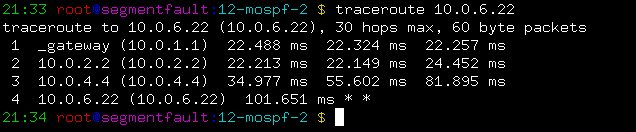
\includegraphics[scale = 0.4]{1.png}
  \caption{运行截图}
\end{figure}


\section*{{\CJKfamily{zhhei}结果分析}}
实验结果正确。
\end{document}


